\chapter{Phase stability and elastic properties study of the Ti-Ta and Ti-Nb systems}

\section{Introduction}

The present chapter is aimed at studying the formation of the metastable phases $\omega$ and $\alpha"$. As shown in chapter 1 Figure \ref{Ch1-figure:tinbelasitc} and \ref{Ch1-figure:titaelastic}, the formation of the $\alpha"$ and $\omega$ phases effects the elastic properties of the implant alloy. Understanding the effect of the metastable phases and at what compositions they form will help with alloy selection and increase the likelihood of finding a suitable alloy for the load-bearing implant appliction. The stabiliy at 0 $^\circ$K of the bcc, hcp, $omega$, $alpha"$ phases is calculated and discussed for the Ti-Ta and Ti-Nb alloys using multiple structures across the entire composition range. The elastic properties of the four phases are then calculated systematically and interaction parameters are introducted using the CALPHAD method, similar to chapter 5, to be able to predict the elastic properties as a function of composition. With an understanding of how the phases effect the elastic properties, a new theoretical framework was introduced in chapter 2 in order to be able to predict the formation of the metastable phases. This chapter uses the new theoretic framework to study Ti and the Ti-Nb system in the bcc, $\omega$ and $\alpha"$ phases. The theoretic framework is used to predict the phase fractions of the metastable phases and the mixed force constants to plot the phonon density of states. In order to ensure the accuracy of the theroretic framework, neutron scattering experiments are completed on 4 different Ti-Nb compositions. The data from the experiments is used to determine the phase fractions and phonon density of states. The results from the neutron scattering are compared with the theoretical results. The determined phase fractions are used to predict the elastic properties and compared with experimental values in literature.

\section{Modeling and Calculations}

\subsection{Computational details}

In the present work the Vienna ab-initio Simulation Package (VASP) \cite{Kresse1996} was employed to calculate the ground state energy and elastic properties of the pure elements and Ti-Nb and Ti-Ta systems in the bcc, hcp, $\omega$, and $\alpha"$ phases. The ion-electron interactions were described using the projector augmented wave (PAW) \cite{Kresse1999,Blochl1994} method and based on the previous work of comparing X-C functionals (Figure \ref{Ch2-figure:PBEvsPW91}) the exchange-correlation functional of the generalized gradient approach depicted by Perdew, Burke, and Ernzerhof (PBE-GGA) was employed \cite{Perdew1996a}. The energy convergence criterion was 10$^{-6}$ eV/atomThe Brillouin zone sampling was done using the $\gamma$-centered Monkhorst-Pack scheme \cite{Monkhorst1976a}. The ground state energy of 330 structures in the bcc phase, across the entire compostition range, were calculated using 8x8x8 k-point meshes. The ground state energy of 21 structures in the hcp phase, across the entire compostition range, were calculated using 10x10x13 k-point meshes. The ground state energy of 73 structures in the $\omega$ phase, across the entire compostition range, were calculated using 13x13x7 k-point meshes. The ground state energy of 33 structures in the $\alpha"$ phase, across the entire compostition range, were calculated using 12x11x10 k-point meshes.The elastic properties were then calculated using a $\pm$0.01 magntiude of strain.

\subsection{Modeling details}

The elastic stiffness constants were modeled using the first-principles based DFT results. The modeling was completed by calculating the difference between the first-principles calculations and a linear extrapolation between pure elements. The differences were then used to fit to the interaction parameters. Due to the limitations within the PARROT module, a mathmatica script was used to fit the interaction parameters. The mathematica script is appended in appendix C. The best fit was found by comparing the fittings obtained with one interaction parameter or with two interaction parameters. The moduli values were than calculated using pycalphad and the code in appendix D and E \cite{Otis2017}.

\section{Results and discussion}

\subsection{First-principles calculations at 0 K}

The phase stability at 0 $^\circ$K is calculated as a function of composition for the Ti-Nb and Ti-Ta systems. Figure \ref{Ch7-figure:tinb0K} shows the relative energy of the bcc, hcp, $\omega$, and $\alpha"$ phases from 100 at. \% Ti to 100 at. \% Nb. The relative energies are calculated similiarliy to the enthalpy of formation in Eq. \ref{eq: hform}, the ground state energies of the pure elements in the SER state are multipled by the composition of the specific structure and then stubtracted from the ground state energy of the structure being studied. Figure \ref{Ch7-figure:titab0K} is the relative energy of the bcc, hcp, $\omega$, and $\alpha"$ phases from 100 at. \% Ti to 100 at. \% Ta. Figure \ref{Ch7-figure:tinb0K} and \ref{Ch7-figure:titab0K} are both at 0 $^\circ$K. The figures show that the bcc and hcp phases are the lowest phases in energy. This shows that the $\omega$ and $\alpha"$ phases are stabilized by entropy.

The Ti-Nb system is chosen to study more in depth due to the experimental work avaliable in the literature which mapped the martensitic transformation temperature for Ti-Nb alloys between the 20 and 30 at. \% Nb is shown in Figure \ref{Ch7-figure:titnbms} \cite{Kim2006}.  

\subsection{Elastic properties}

For the Ti-Nb system, the elastic stiffness constants of the bcc, hcp, $\alpha"$, and $\omega$ phases are calculated. The calculations of the bcc phase were completed and discussed in chpater 5. Figure \ref{Ch7-figure:adpelas1} and \ref{Ch7-figure:adpelas2} plots the elastic stiffness constants, $C_{11}$, $C_{12}$, $C_{13}$, $C_{22}$, $C_{23}$, $C_{33}$, $C_{44}$, $C_{55}$, and $C_{66}$, for the $\alpha"$ phase. The $C_{11}$, $C_{22}$, $C_{23}$, $C_{55}$, and $C_{66}$ values all start off decreasing, then being to increase in value and finally decrease in value from pure Ti to pure Nb. The $C_{12}$ and $C_{13}$ values all start off increasing, then being to decrease in value and finally increase in value from pure Ti to pure Nb. The $C_{33}$ values decrease and then increase in value from pure Ti to pure Nb. The $C_{44}$ values start off increasing and then decrease in value from pure Ti to pure Nb. 

Figure \ref{Ch7-figure:omegae1} plots the elastic stiffness constants, $C_{11}$, $C_{12}$, $C_{13}$, $C_{33}$, and $C_{44}$, for the $\omega$ phase. The $C_{11}$ and $C_{33}$ values all start off increasing and then decreasing from pure Ti to pure Nb. The $C_{11}$ values all start off decreasing and then increase from pure Ti to pure Nb. The $C_{12}$ increases, decreases and then increases in values from pure Ti to pure Nb. The $C_{33}$ values start off dcreasing then increase and then decrease again from pure Ti to pure Nb. 

Figure \ref{Ch7-figure:hcpe1} plots the elastic stiffness constants, $C_{11}$, $C_{12}$, $C_{13}$, $C_{33}$, and $C_{44}$, for the hcp phase. The $C_{12}$, $C_{13}$ and $C_{33}$ values all start off decreasing, then increase and then decrease from pure Ti to pure Nb. The $C_{11}$ values decrease from pure Ti to pure Nb. The $C_{44}$ values increase, decrease and then increase from pure Ti to pure Nb. 

The calculated elastic stiffness constants are listed in Table \ref{Ch7-table:tinbdata}. From the elastic stiffness constants, the Young's moduli values are calculated as a function of composition and are plotted in Figure \ref{Ch7-figure:tinbelastic}. The dotted lines are the fittings that use the interaction parameters in Table \ref{Ch7-table:intpara}. The calculations show that the Young's moduli, for the hcp phase, decrease in value until around 80 at. \% Nb and then increase from 80 at. \% Nb to pure Nb. The Young's moduli, for the omega phase, follows the same trend as the hcp phase. The $E$ vlaues decrease from putre Ti to around 60 at. \% Nb and then increase from 60 at. \% Nb to pure Nb. The $E$ values, for the bcc phase, increase from pure Ti to pure Nb. The $E$ values, for the $\alpha"$ phase, decrease from pure Ti to around 20 at. \% Nb, then increase from 10 at. \% Nb to 70 at. \% Nb and then decrease from 70 at. \% Nb to pure Nb. The $E$ values for the hcp, $\omega$, and bcc phases all go negative at some point. Based on Born's criteria, a negative Young's modulus can indicate that the phase is not stable at that composition. From Figure \ref{Ch7-figure:tinbelastic}, it can be seen that the $E$ values of the $alpha"$ phase are higher than the hcp or bcc pahses. This explains why in Figure \ref{Ch1-figure:tinbelasitc} the experimental Young's moduli increase in value with the formation of the metastable. 

At least four different authors have experimentally determined the $E$ of various Ti-Nb alloys at different compositions, which are plotted in Figure \ref{Ch1-figure:tinbelasitc}, \cite{Friak2012,Timoshevskii2011,Friak2012,Karre2015}. Ozaki et al. \cite{Ozaki2004} showed the same results discussed earlier that at certain compositions quenched samples formed bcc and $\alpha"$ while the cooled samples formed bcc and $\omega$. There was more experimental results for the quenched samples which is why present work reviewed this data and averaged the $E$ values at the same compositions. The full experimental results reviewed are listed in appendix F and the averaged experimental values are listed in Table \ref{Ch7-table:elasexptdata}. From these experiments, some of the phase fractions were determined \cite{Friak2012} and those phase fractions are listed in Table \ref{Ch7-table:elasexptdata}. For the compositions were the phase fractions were not determined, we extrapolated an estimated phase fractions, those phase fractions are in italics in order to differentiate from a prediction and a measure phase fraction.  Based on these phase fractions and the interaction parameters in Table \ref{Ch7-table:intpara}, the rule of mixtures is used to predict the Young's moduli and compared with the experimentally determined $E$. The rule of mixtures is experssed by: 

%%
\begin{equation}
\label{eq:ruleofmix}
E_{c}=x_{p1}E_{p1}+x_{p2}E_{p2}
\end{equation}
%%

\noindent where $x_{p1}$ and $x_{p2}$ are the phase fractions of phase 1 and phase 2. $E_{p1}$ and $E_{p2}$ are the elastic modulus of the alloys in phase 1 and phase 2. Based on the data up until 10 at. \% Nb the samples are 100 \% hcp and the predicted $E$ vary, on average, from the experimental $E$ by 7.7 GPa. From 10 at. \% Nb to 30 at. \% Nb the $\alpha"$ and bcc phases formed. The exact phase fraction of the bcc phase was measured by Friak et al. for the 10, 20, 25, and 30 at. \% Nb samples. An extrapolation from these values is used for the phase fractions of the remaining alloys in this composition range. Using the phase fractions and rule of mixtures, the prediced $E$ varies, on average, from the experimental $E$ by 0.52 GPa. If the alloys had been assumed to be a bcc and hcp mixture, as the CALPHAD predictions tell us, the predicted $E$ would vary, on average, from the experimental $E$ by 22 GPa. Above 33 at. \% Nb the samples are all bcc phase. The predicted $E$ vary, on average, from the experimental $E$ by 7 GPa. Overall, the variances are quite small when compared to the variance seen in the experiments. As seen in appendix F, the experimental $E$ values of pure Ti in the hcp phase vary by 24 GPa. The variance between the predicted $E$ and experimental $E$ can be attributed to the fact that the predicted $E$ are at 0 $^\circ$K and the experimental $E$ are at 300 $^\circ$K. Based on the comparison, it is seen that if the phase fraction of the metastable phases can be predicted than the database can be used with the rule of mixtures to accurately predict the elastic properites. 

\subsection{Neutron scattering results}

\subsubsection{Phonon density of states at 300 K}

The phonon density of states was obtained at 300 $^\circ$K for each set of samples at each Nb composition. The phonon density of states are plotted in Figure \ref{Ch7-figure:50dos20}, \ref{Ch7-figure:50dos18}, \ref{Ch7-figure:50dos12}, \ref{Ch7-figure:50dos10}. The samples at the same composition are plotted together for comparison. The phonon density of states of the slow cooled samples, that should contain the bcc and $\omega$ phases, are plotted with dashed lines and the phonon density of states of the quenced samples, that should contain the bcc and $\alpha "$ phases, are plotted with solid lines. The fact that the different samples show different phonon DOS means that the quenching versus slow cooling worked and the samples should have different phases. In order to investigate the difference of the phonon DOS further the entropy of each sample was calculated from the phonon DOS ($g(E)$):

%%
\begin{equation}
\label{eq:phononentropy}
S_{vib} = 3 k_{B} \int_{0}^{E_{max}} \left[ \left( n+1 \right) ln\left(n+1\right) -n ln\left(n\right) \right] g(E) dE
\end{equation}
%%

\noindent where $n$ is the Bose-Einstein occupation factor \cite{Budai2014}. The entropy difference between the alloys at the same compositions is plotted in \ref{Ch7-figure:ediff}. The figure shows that the entropy difference increases from 10 mol \% Nb to 20 mol \% Nb. The increase in entropy with increasing Nb content makes sense when looking at Figure \ref{Ch1-figure:tinbelasitc}. The figure and previous research shows that the $\alpha"$ and $\omega$ phases form from approximately 10 mol \% to 35 mol \% Nb. At 10 mol \% Nb, only a small amount of the metastable phases form which is why the experimentally determined elastic properties still line up well with the theoretically obtained elastic properites. This is supported by the lower entropy difference between the two 10 mol \% Nb alloys. However, closer to 20 mol \% Nb, Figure \ref{Ch7-figure:tinbelastic} shows that the experimental Young's moduli is higher than computationally determined Young's moduli. Research showed that the phase fractions of the metastable phase is larger at this composition than the three other compositions studied in this work. This is supported by the larger difference in entropy at 20 mol \% Nb.

\subsubsection{Diffraction patterns at 300 K}

The diffraction patterns for each alloy are plotted in Figure \ref{Ch7-figure:50diff20}, \ref{Ch7-figure:50diff18}, \ref{Ch7-figure:50diff12} \ref{Ch7-figure:50diff10}. The slow cooled samples are plotted as solid lines and the quenched samples are plotted as dashed lines. The diffraction patterns plot the Q vs. the intensity. Using a different neutron scattering technique or x-ray diffraction would lead to better diffraction patterns and more accurate predictions of the phase stability. The plots are compared with known diffraction patterns of Ti and Nb in the four phases to determine an approximation of the phase fractions. The determined phase fractions of each alloy are listed in Table \ref{Ch7-table:phasefrac}. The analysis shows that the quenched samples formed 0.12, 0.20, 0.57 and 0.70 phase fraction of bcc for the 10, 12, 18 and 20 at. \% Nb samples, respectively. The slow cooled samples showed 0.2, 0.3, 0.6, 0.7 phase fraction of the bcc phase for the 10, 12, 18, and 20 at. \% Nb samples, respectively. The phase fractions for the 10 and 20 at. \% Nb quenched samples compares well with the fractions determined by Friak et al. \cite{Friak2012} shown in Table \ref{Ch7-table:elasexptdata}. 

\subsection{Partition function approach results}

The implementation of the new theoretical framework is ongoing. Due to the difficulty of implementing the theoretic framework, we began by calculating pure Ti. The energy is being mapped for Ti in the bcc, $\omega$, $\alpha"$ and hcp phases looking for the energy minima. Quasiharmonic phonon calculations will be completed on the structures at the lowest energy minima points. The helmholtz energy results and eigenvalues from these calcualtions will be used in Eq. \ref{eq: combinedhelmholtz}, \ref{eq: combinedhelmholtz2}, \ref{eq: zc}, and \ref{eq: zi}. Using the calculation of entropy, from the combined helmholtz, this work should more accurately predict Ti in the bcc phase. Once the work has been shown to be accurate for pure Ti, it will be extended to the Ti-Nb binary system and compared to the neutron scattering results.

\section{Conclusion}

The present study systematically calculates the elastic stiffness constants and Young's moduli of the Ti-Nb system in the bcc, hcp, $\omega$, and $\alpha"$ phases. The general CALPHAD modeling approach is used to fit binary interaction parameters. The $E$ values were similar for the hcp and $\omega$ phase which makes sense since they both have hexagonal symmetry. The $\alpha"$ phase has $E$ values that are higher than the other three phase which explains why when formed the $E$ increases. Experiments showed that up to 10 at. \% Nb the samples formed solely the hcp phase and the database predicts the $E$ values by an average variance of 8 GPa from the experimental $E$. The samples from 10 at. \% Nb to 30 at. \% Nb formed both the bcc and $\alpha"$ or $\omega$ phases. If the samples are slow cooled then the samples form the bcc and $\omega$ phases. If the samples are quenched they form the bcc and $\alpha"$ phases. Using experimentally determined phase fractions and the rule of mixtures, the database accurately predicts the $E$ values by an average variance of 0.52 GPa when compared with the experimental $E$ values. At Nb concentrations greater than 30 at. \% Nb form solely the bcc phase and the database predicts the $E$ values by an average variance of 7 GPa from the experimental $E$ values. The phonon DOS at 300 $^\circ$K differences between the slow cooled and quenced samples especially when looking at the entropy difference between the samples. Diffraction patterns from ARCS are diffcult to fit but the phase fractions are approximated. The implementation of the new theoretic framework is ongoing but from the results here, if the phase fractions of the metastable phases can be predicted then the elastic database can accurately assess the Young's moduli and elastic stiffness constants. 

\newpage
\begin{longtable}[H]{ c c c c c c c c c c }
	\caption{First-principles calculations of the elastic stiffness constants in GPa for different atomic percent compositions in the $\alpha"$, bcc, hcp, and $\omega$  phases in the Ti-Nb system at 0 $^\circ$K.} 	\label{Ch7-table:tinbdata} \\
	\hline
	Ti$_{1-b}$Nb$_b$ & c$_{11}$ & c$_{12}$ & c$_{13}$ & c$_{22}$ & c$_{23}$ & c$_{33}$ & c$_{44}$ & c$_{55}$ & c$_{66}$\\
	\hline
	\endhead
	\hline
	\endfoot
	\multicolumn{10}{c}{$\alpha"$}\\
	\hline
	Ti & 198 & 69 & 84 & 197 & 84 & 189 & 40 & 40 & 63 \\		
	TiNb$_{3}$ & 106 & 112 & 123 & 152 & 45 & 138 & 25 & 17 & 38 \\
	TiNb$_{13}$ & 171 & 88 & 105 & 171 & 67 & 170 & 47 & 13 & 43 \\
	TiNb$_{94}$ & 307 & 94 & 119 & 248 & 143 & 214 & 31 & -24 & 13 \\
	TiNb$_{97}$ & 307 & 88 & 115 & 232 & 124 & 284 & 59 & -58 & 8 \\
	TiNb$_{98}$ & 293 & 88 & 115 & 232 & 124 & 284 & 59 & -58 & 8 \\
	Nb & 306 & 88 & 125 & 240 & 135 & 284 & 47 & -69 & 9 \\
	\hline
	\multicolumn{10}{c}{bcc}\\
	\hline
	Ti & 93 & 115 & - & - & - & - & 41 & - & - \\		
	TiNb$_{2}$ & 93 & 115 & - & - & - & - & 35 & - & - \\
	TiNb$_{13}$ & 116 & 116 & - & - & - & - & 37 & - & - \\
	TiNb$_{25}$ & 140 & 116 & - & - & - & - & 34 & - & - \\
	TiNb$_{50}$ & 181 & 121 & - & - & - & - & 31 & - & - \\
	TiNb$_{75}$ & 208 & 130 & - & - & - & - & 15 & - & - \\
	TiNb$_{94}$ & 242 & 134 & - & - & - & - & 18 & - & - \\
	TiNb$_{98}$ & 242 & 134 & - & - & - & - & 18 & - & - \\
	Nb & 245 & 144 & - & - & - & - & 27 & - & - \\
	\hline
	\multicolumn{10}{c}{hcp}\\
	\hline
	Ti & 175 & 88 & 80 & - & - & 190 & 41 & - & - \\		
	TiNb$_{2}$ & 79 & -44 & -38 & - & - & 73 & 45 & - & - \\
	TiNb$_{13}$ & A & B & C & - & - & D & E & - & - \\
	TiNb$_{25}$ & 156 & 113 & 104 & - & - & 200 & 13 & - & - \\
	TiNb$_{50}$ & 124 & 151 & 135 & - & - & 185 & -19 & - & - \\
	TiNb$_{75}$ & 76 & 213 & 156 & - & - & 173 & -61 & - & - \\
	TiNb$_{94}$ & 15 & 289 & 177 & - & - & 163 & -104 & - & - \\
	TiNb$_{98}$ & 34 & 280 & 185 & - & - & 145 & -106 & - & - \\
	Nb & 24 & 18 & 11 & - & - & 25 & -6 & - & - \\
	\hline
	\multicolumn{10}{c}{$\omega$}\\
	Ti & 194 & 87 & 61 & - & - & 246 & 54 & - & - \\
	TiNb$_{2}$ & 187 & 87 & 63 & - & - & 250 & 50 & - & - \\
	TiNb$_{13}$ & 171 & 89 & 83 & - & - & 165 & 30 & - & - \\
	TiNb$_{94}$ & 240 & 90 & 142 & - & - & 234 & -22 & - & - \\
	TiNb$_{98}$ & 242 & 88 & 120 & - & - & 270 & -5 & - & - \\
	Nb & 243 & 181 & 110 & - & - & 212 & -55 & - & - \\
	\hline
\end{longtable}
%%%

\newpage
\newpage
\begin{table}[H]
	\caption{Evaluated interaction parameters $L_0$ and $L_1$, using Eq. \ref{eq: elastic}, for the elastic stiffness constants of the bcc, hcp, $\alpha"$ and $\omega$ phases in the Ti-Nb systems.}
	\centering
	\begin{tabular}{ c c c c c c }
		\hline
		Alloy & Interaction Parameter & $\alpha"$ & bcc & hcp & $\omega$\\
		\hline
		c$_{11}$ & $L_{0}$ & -102.443 & 40.4555 & 92.0107 & -142.979 \\
		& $L_{1}$ & 606.748 & - & 126.357 & 159.767 \\
		c$_{12}$ & $L_{0}$ & 97.3105 & -32.3885 & 719.463 & -888.25 \\
		& $L_{1}$ & -186.214 & - & 1322.75 & -1074.08 \\
		c$_{13}$ & $L_{0}$ & -11.5368 & N/A & 541.702 & 349.337 \\
		& $L_{1}$ & -307.745 & N/A & 906.397 & 275.297 \\
		c$_{22}$ & $L_{0}$ & -100.063 & N/A & N/A & N/A \\
		& $L_{1}$ & 355.649 & N/A & N/A & N/A \\
		c$_{23}$ & $L_{0}$ & -75.1048 & N/A & N/A & N/A \\
		& $L_{1}$ & 283.22 & N/A & N/A & N/A \\
		c$_{33}$ & $L_{0}$ & -468.983 & N/A & 481.962 & -100.909 \\
		& $L_{1}$ & -114.152 & N/A & 665.306 & 733.448 \\
		c$_{44}$ & $L_{0}$ & 14.125 & -41.5375 & -266.658 & 263.258 \\
		& $L_{1}$ & - & -41.9528 & -416.274 & 475.336 \\
		c$_{55}$ & $L_{0}$ & 204.71 & N/A & N/A & N/A \\
		& $L_{1}$ & 479.179 & N/A & N/A & N/A \\
		c$_{66}$ & $L_{0}$ & -59.1357 & N/A & N/A & N/A \\
		& $L_{1}$ & 139.625 & N/A & N/A & N/A \\
		\hline
	\end{tabular}
	\label{Ch7-table:intpara}
\end{table}
\clearpage
%%%

\newpage
\begin{table}[H]
	\caption{Phase fractions and experimetally determined $E$ compared with the predicted $E$ using the rule of mixtures and interaction parameters in Table \ref{Ch7-table:intpara} for the Ti-Nb system.}
	\centering
	\begin{tabular}{ c c c c}
		\hline
		x(Nb) & Phase Fraction & Expt $E$ & Calc $E$\\
		\hline
		0.00 & all hcp & 118.31 & 123.8\\
		0.01 & all hcp & 112.52 & 117.7\\
		0.02 & all hcp & 108.33 & 112.0\\
		0.05 & all hcp & 79.47 & 94.9\\
		0.08 & all hcp & 66.41 & 78.4\\
		0.09 & all hcp & 68.73 & 73.1\\
		0.10 & 0.06 BCC/0.94 $\alpha"$ & 84.64 & 95.89\\
		0.11 & $0.15 BCC/0.94 \alpha"$ & 78.72 & 88.19\\
		0.18 & $0.45 BCC/0.94 \alpha"$ & 93.02 & 70.08\\
		0.19 & $0.49 BCC/0.94 \alpha"$ & 64.26 & 68.65\\
		0.20 & 0.60 BCC/0.94 $\alpha"$ & 77.62 & 65.74\\
		0.22 & $0.63 BCC/0.94 \alpha"$ & 70.90 & 67.44\\
		0.23 & $0.67 BCC/0.94 \alpha"$ & 75.85 & 67.00\\
		0.24 & $0.71 BCC/0.94 \alpha"$ & 61.11 & 66.63\\
		0.25 & 0.81 BCC/0.94 $\alpha"$ & 72.52 & 66.10\\
		0.26 & $0.80 BCC/0.94 \alpha"$ & 66.61 & 66.23\\
		0.27 & $0.84 BCC/0.94 \alpha"$ & 54.61 & 66.98\\
		0.29 & $0.91 BCC/0.94 \alpha"$ & 62.13 & 66.16\\
		0.30 & 0.90 BCC/0.94 $\alpha"$ & 68.11 & 68.21\\
		0.34 & all bcc & 77.47 & 66.69\\
		0.36 & all bcc & 73.78 & 69.00\\
		0.39 & all bcc & 76.62 & 69.81\\
		0.43 & all bcc & 84.05 & 69.77\\
		\hline
	\end{tabular}
	\label{Ch7-table:elasexptdata}
\end{table}
\clearpage
%%%

\newpage
\begin{table}[H]
	\caption{Phase fractions determined from the diffraction patterns for the Ti-Nb alloys.}
	\centering
	\begin{tabular}{ c c c c c }
		\hline
		Alloy & x(Nb) & \multicolumn{3}{c}{Phase Fraction} \\
		&  & bcc & $\omega$ & $\alpha"$ \\
		\hline
		Q-TiNb$_{10}$ & 0.10 & 0.12 & - & 0.88 \\
		Q-TiNb$_{12}$ & 0.12 & 0.20 & - & 0.80 \\
		Q-TiNb$_{18}$ & 0.18 & 0.57 & - & 0.43 \\
		Q-TiNb$_{20}$ & 0.20 & 0.70 & - & 0.3 \\
		SC-TiNb$_{10}$ & 0.10 & 0.20 & 0.8 & - \\
		SC-TiNb$_{12}$ & 0.12 & 0.30 & 0.7 & - \\
		SC-TiNb$_{18}$ & 0.18 & 0.60 & 0.4 & - \\
		SC-TiNb$_{20}$ & 0.20 & 0.70 & 0.3 & - \\
		\hline
	\end{tabular}
	\label{Ch7-table:phasefrac}
\end{table}
\clearpage
%%%

\pagebreak
\begin{figure}[H]
	\centering
	\includegraphics[width=\textwidth]{Chapter-7/Figures/tinb0k.png}
	\caption{Relative energy of the bcc, hcp, $\omega$, $\alpha"$ phases in the Ti-Nb system are plotted from 100 at. \% Ti to 100 at. \% Nb.}
	\label{Ch7-figure:tinb0K}
\end{figure}

\pagebreak
\begin{figure}[H]
	\centering
	\includegraphics[width=\textwidth]{Chapter-7/Figures/tita0k.png}
	\caption{Relative energy of the bcc, hcp, $\omega$, $\alpha"$ phases in the Ti-Ta system are plotted from 100 at. \% Ti to 100 at. \% Ta.}
	\label{Ch7-figure:titab0K}
\end{figure}

\pagebreak
\begin{figure}[H]
	\centering
	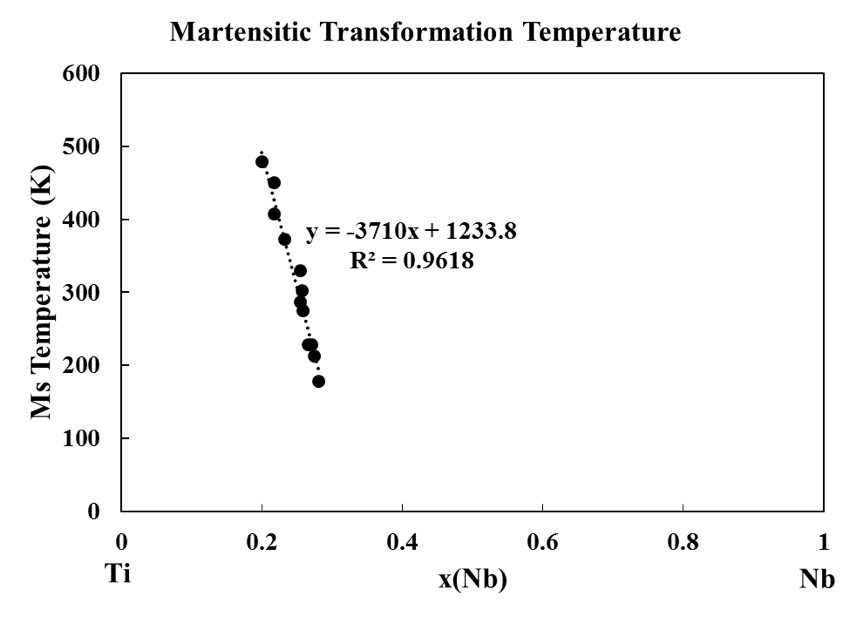
\includegraphics[width=\textwidth]{Chapter-7/Figures/tinbms.png}
	\caption{Martensitic transformation temperature is plotted versus the Ti-Nb composition.}
	\label{Ch7-figure:titnbms}
\end{figure}

\pagebreak
\begin{figure}[H]
	\centering
	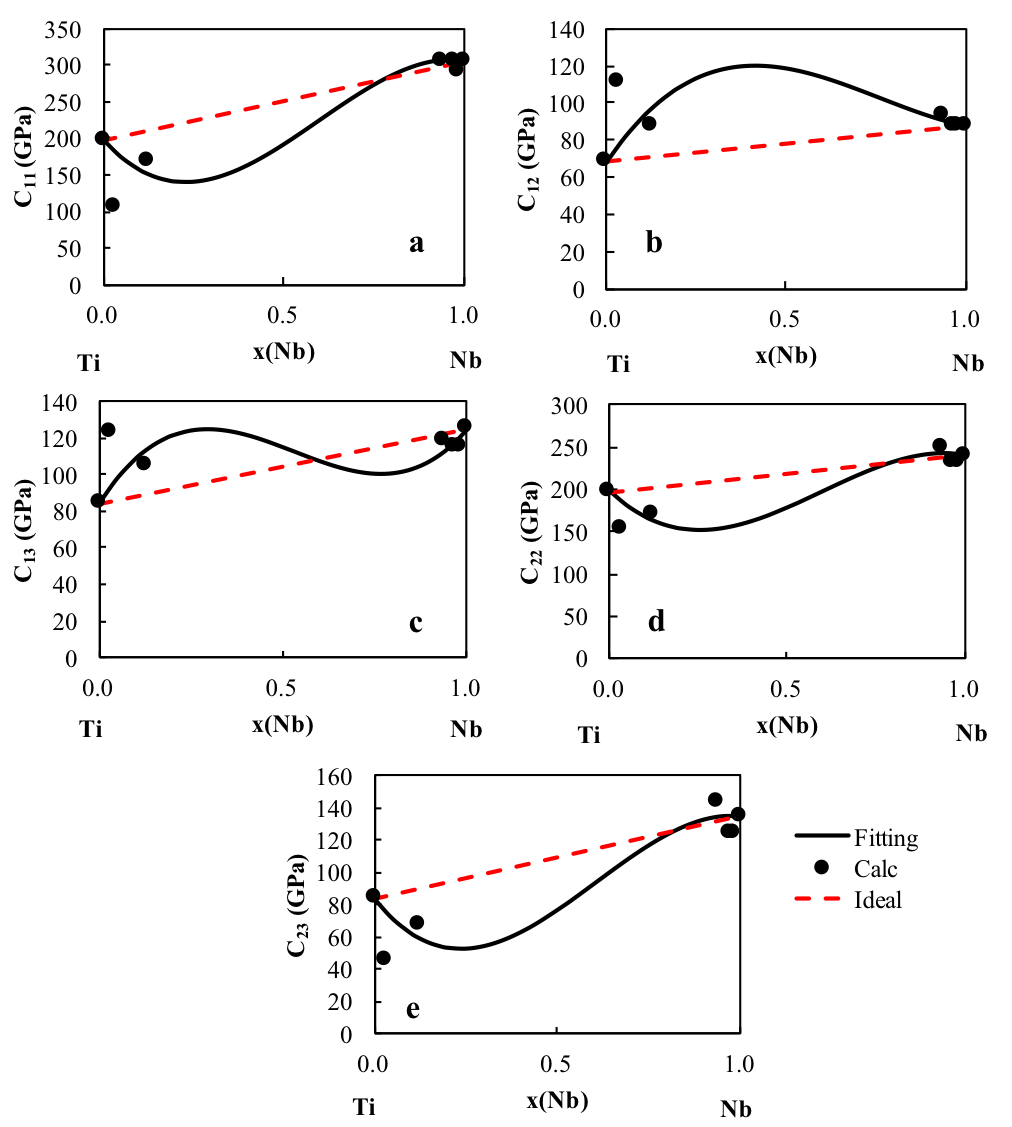
\includegraphics[width=\textwidth]{Chapter-7/Figures/adpe1.png}
	\caption{Calculated $C_{11}$, $C_{12}$, $C_{13}$, and $C_{22}$ values (circles) plotted as well as the pure element extrapolation (red dashed line) and the present modeling (black dashed line) for five of the elastic stiffness constants of Ti-Nb in the $\alpha"$ phase.}
	\label{Ch7-figure:adpelas1}
\end{figure}

\pagebreak
\begin{figure}[H]
	\centering
	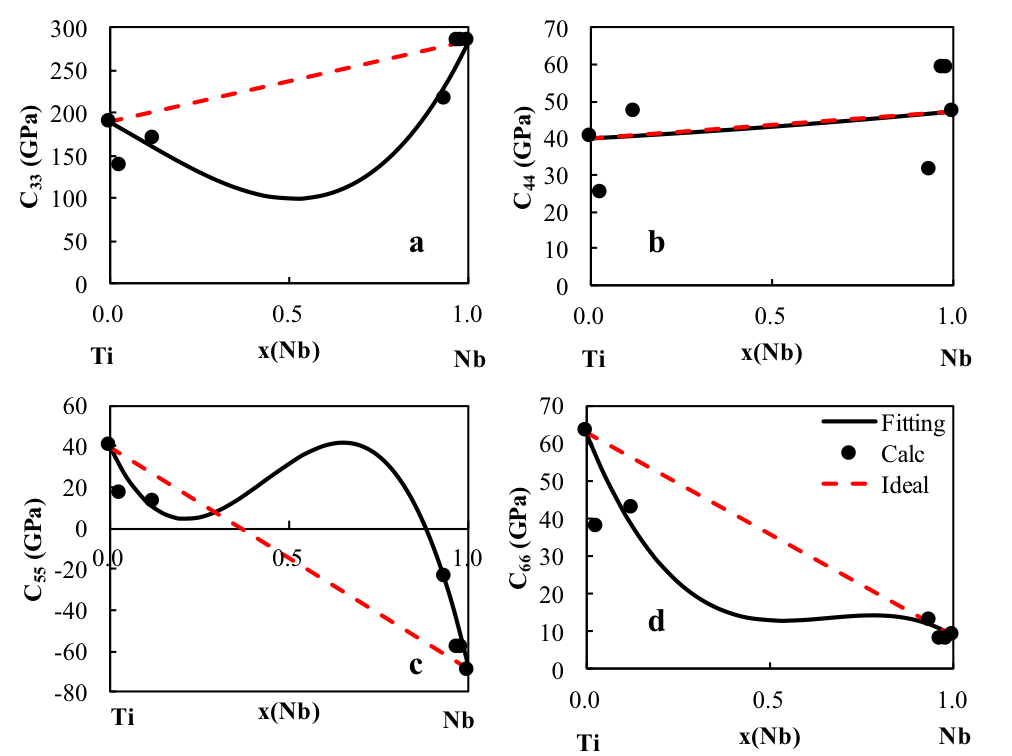
\includegraphics[width=\textwidth]{Chapter-7/Figures/adpe2.png}
	\caption{Calculated $C_{23}$, $C_{33}$, $C_{44}$, $C_{55}$, and $C_{66}$ values (circles) plotted as well as the pure element extrapolation (red dashed line) and the present modeling (black dashed line) for four of the elastic stiffness constants of Ti-Nb in the $\alpha"$ phase.}
	\label{Ch7-figure:adpelas2}
\end{figure}

\pagebreak
\begin{figure}[H]
	\centering
	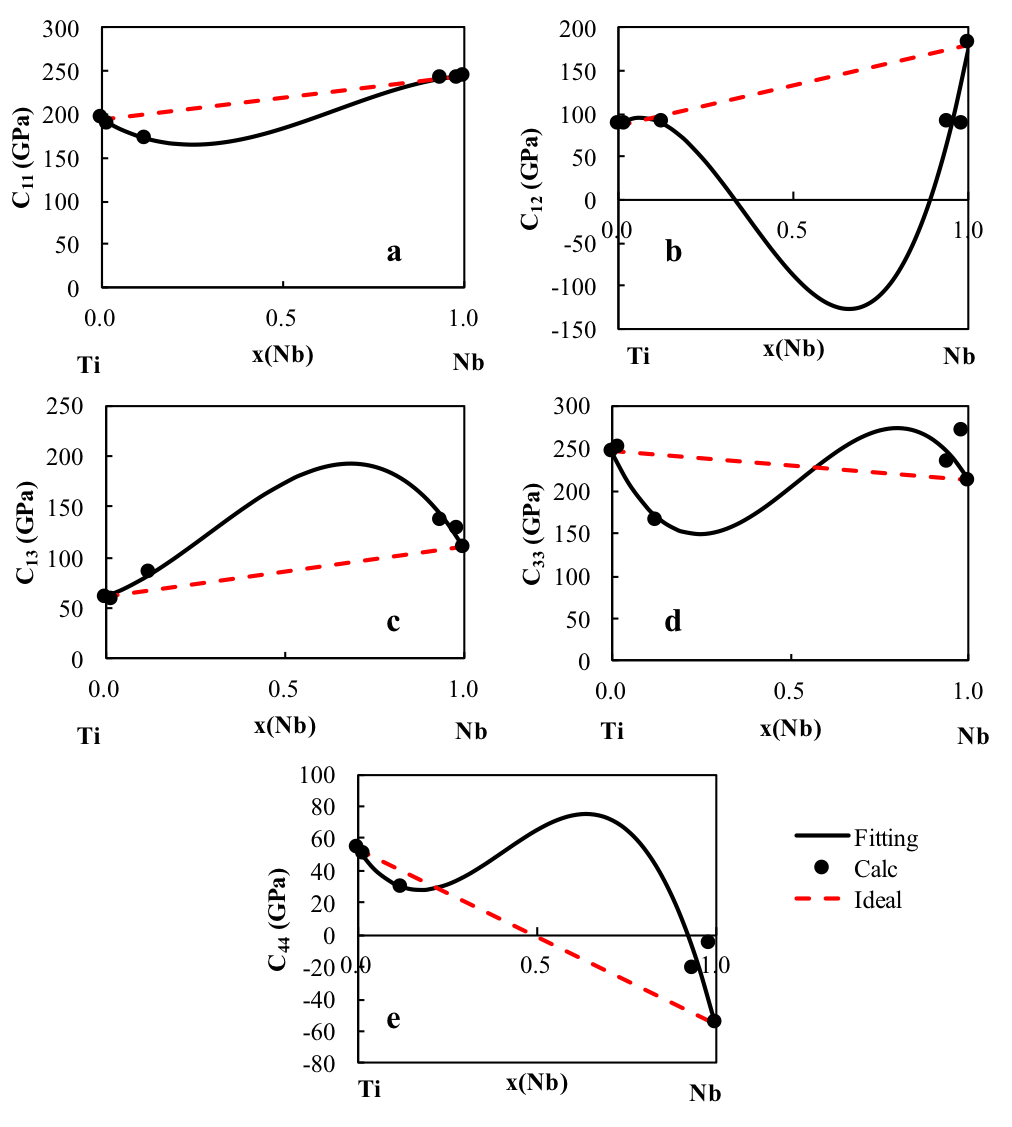
\includegraphics[width=\textwidth]{Chapter-7/Figures/omegae1.png}
	\caption{Calculated $C_{11}$, $C_{12}$, $C_{13}$, $C_{33}$, and $C_{44}$ values (circles) plotted as well as the pure element extrapolation (red dashed line) and the present modeling (black dashed line) for the elastic stiffness constants of Ti-Nb in the $\omega$ phase.}
	\label{Ch7-figure:omegae1}
\end{figure}

\pagebreak
\begin{figure}[H]
	\centering
	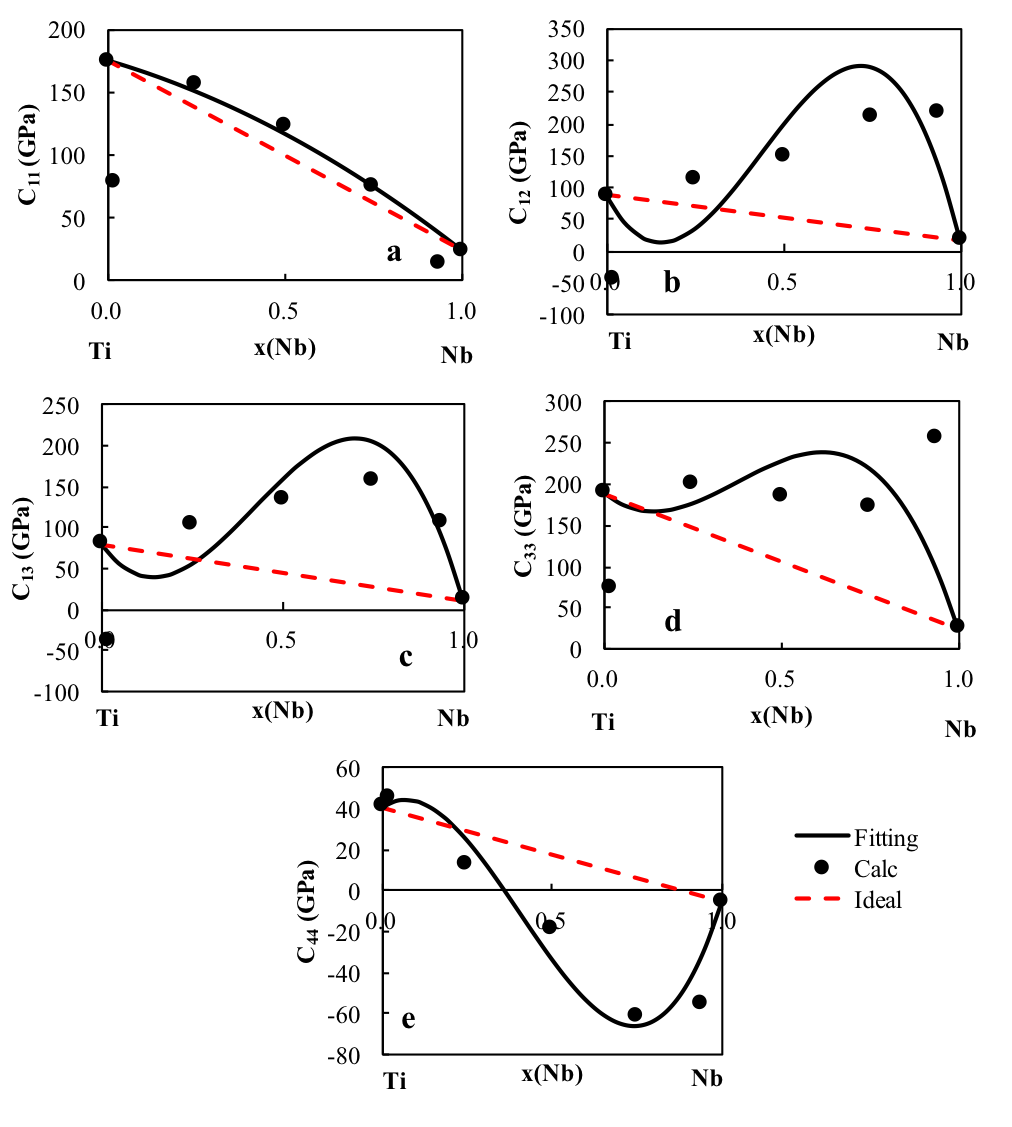
\includegraphics[width=\textwidth]{Chapter-7/Figures/hcpe1.png}
	\caption{Calculated $C_{11}$, $C_{12}$, $C_{13}$, $C_{33}$, and $C_{44}$ values (circles) plotted as well as the pure element extrapolation (red dashed line) and the present modeling (black dashed line) for the elastic stiffness constants of Ti-Nb in the hcp phase.}
	\label{Ch7-figure:hcpe1}
\end{figure}

\pagebreak
\begin{figure}[H]
	\centering
	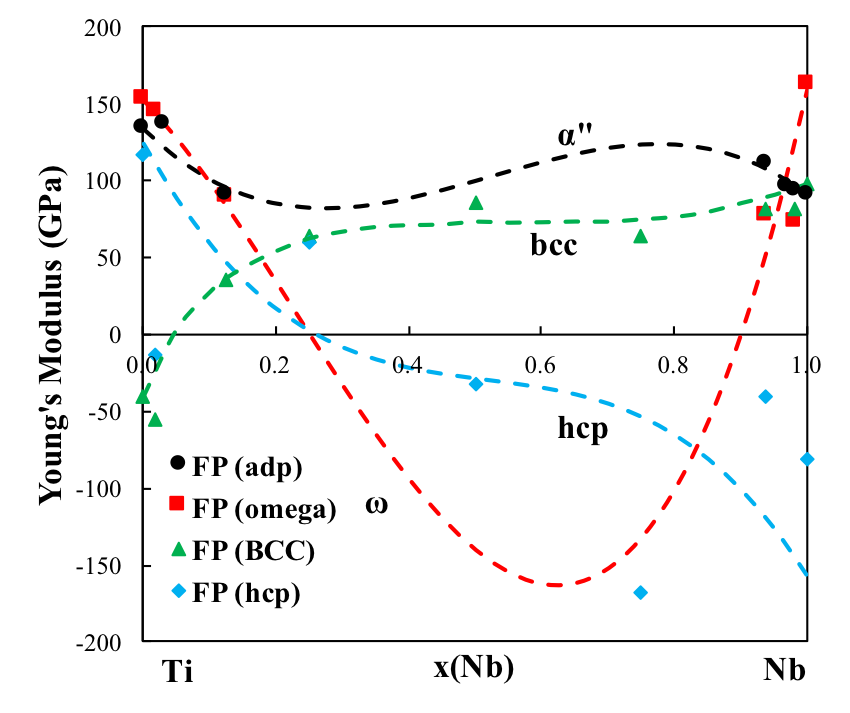
\includegraphics[width=\textwidth]{Chapter-7/Figures/tinbelastic.png}
	\caption{Eelastic properites of the bcc, hcp, $\omega$, $\alpha"$ phases in the Ti-Nb system calculated from first-principles based on DFT are plotted as symbols. The CALPHAD fitting are plotted as the dashed lines. The figure is plotted from 100 at. \% Ti to 100 at. \% Nb.}
	\label{Ch7-figure:tinbelastic}
\end{figure}

\pagebreak
\begin{figure}[H]
	\centering
	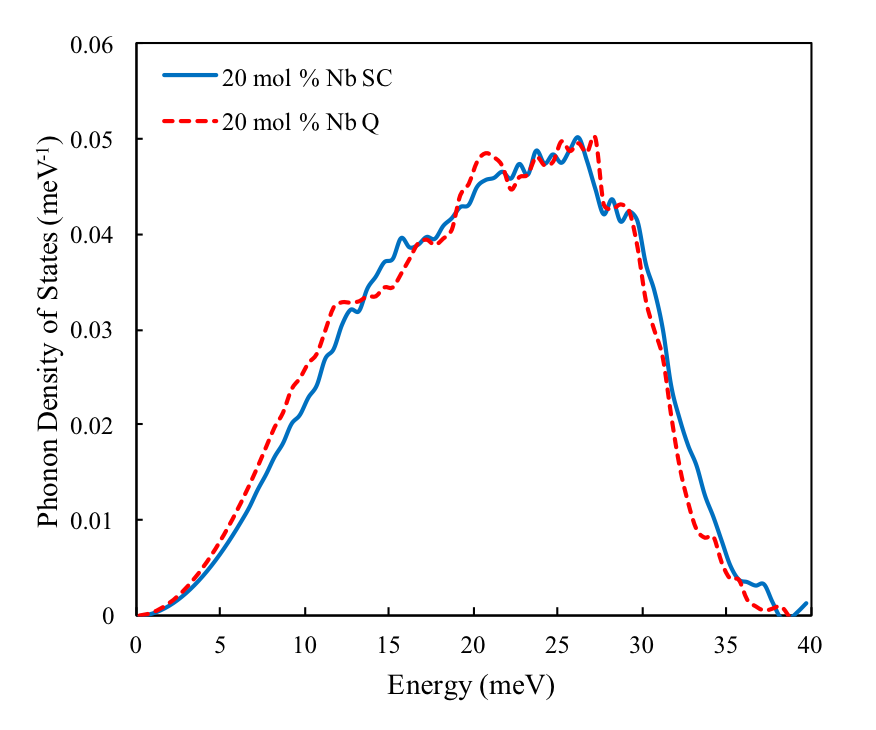
\includegraphics[width=\textwidth]{Chapter-7/Figures/50dos20.png}
	\caption{Phonon density of states is plotted for the TiNb alloy at 20 at. \% Nb. The dashed line represents the slow cooled sample while the solid line represents the quenched sample.}
	\label{Ch7-figure:50dos20}
\end{figure}

\pagebreak
\begin{figure}[H]
	\centering
	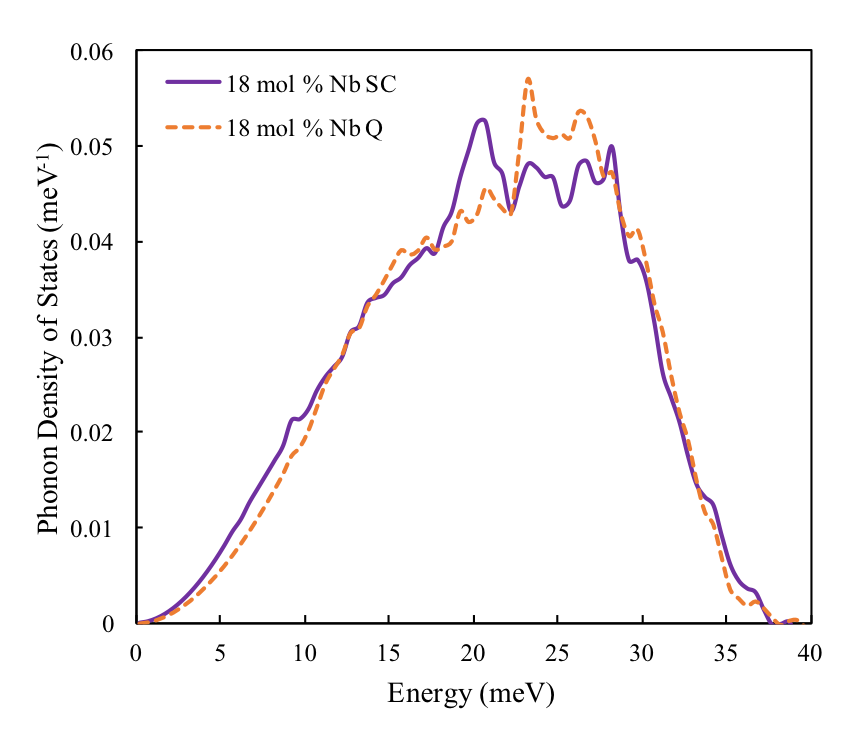
\includegraphics[width=\textwidth]{Chapter-7/Figures/50dos18.png}
	\caption{Phonon density of states is plotted for the TiNb alloy at 18 at. \% Nb. The dashed line represents the slow cooled sample while the solid line represents the quenched sample.}
	\label{Ch7-figure:50dos18}
\end{figure}

\pagebreak
\begin{figure}[H]
	\centering
	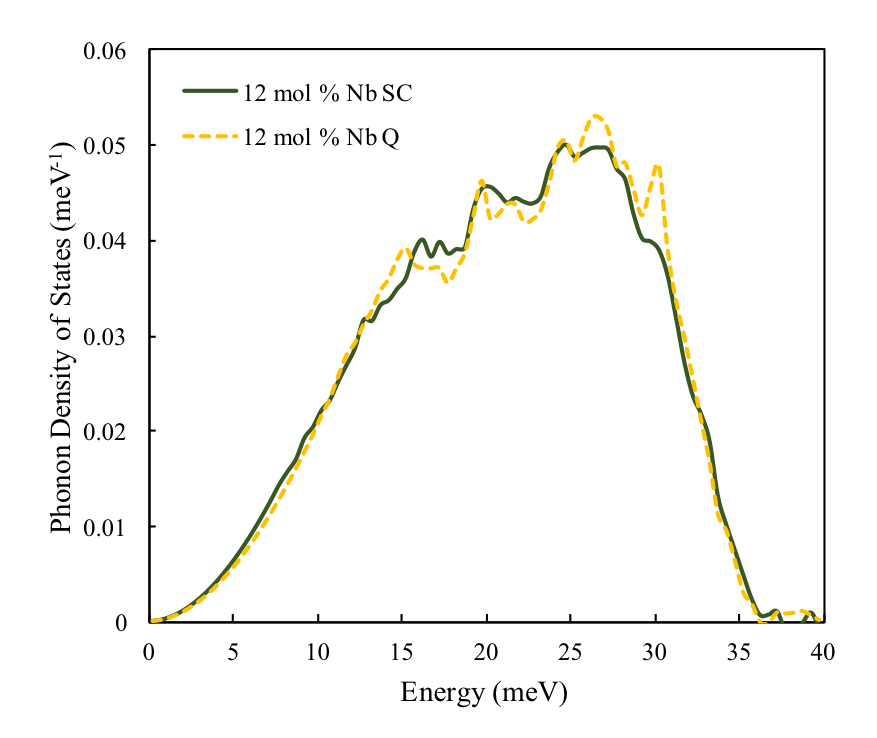
\includegraphics[width=\textwidth]{Chapter-7/Figures/50dos12.png}
	\caption{Phonon density of states is plotted for the TiNb alloy at 12 at. \% Nb. The dashed line represents the slow cooled sample while the solid line represents the quenched sample.}
	\label{Ch7-figure:50dos12}
\end{figure}

\pagebreak
\begin{figure}[H]
	\centering
	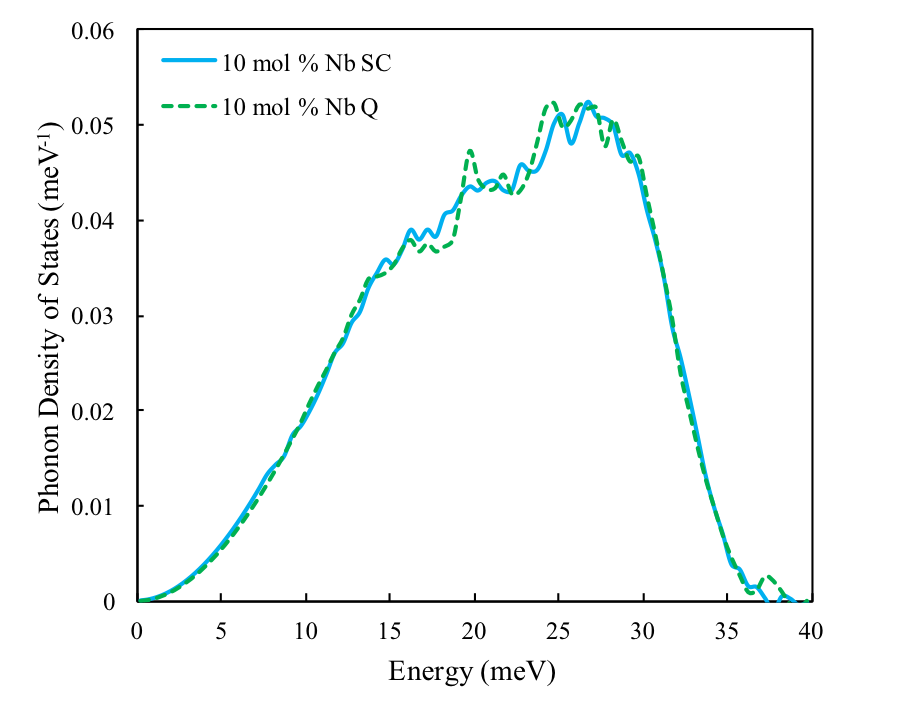
\includegraphics[width=\textwidth]{Chapter-7/Figures/50dos10.png}
	\caption{Phonon density of states is plotted for the TiNb alloy at 10 at. \% Nb. The dashed line represents the slow cooled sample while the solid line represents the quenched sample.}
	\label{Ch7-figure:50dos10}
\end{figure}

\pagebreak
\begin{figure}[H]
	\centering
	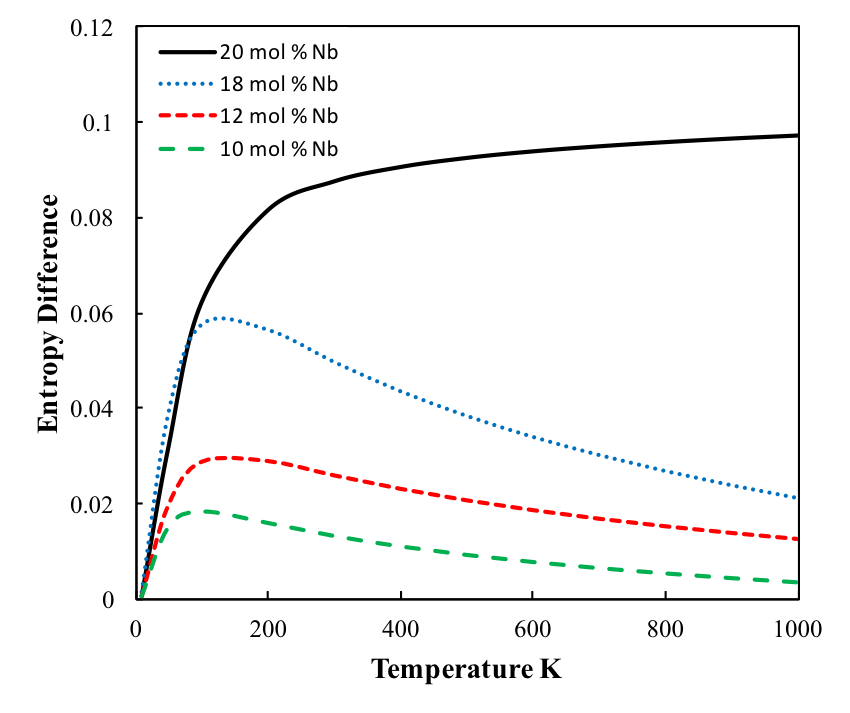
\includegraphics[width=\textwidth]{Chapter-7/Figures/ediff.png}
	\caption{Entropy difference between the Ti-Nb alloys with the same alloy composition is plotted as a function of temperature.}
	\label{Ch7-figure:ediff}
\end{figure}

\pagebreak
\begin{figure}[H]
	\centering
	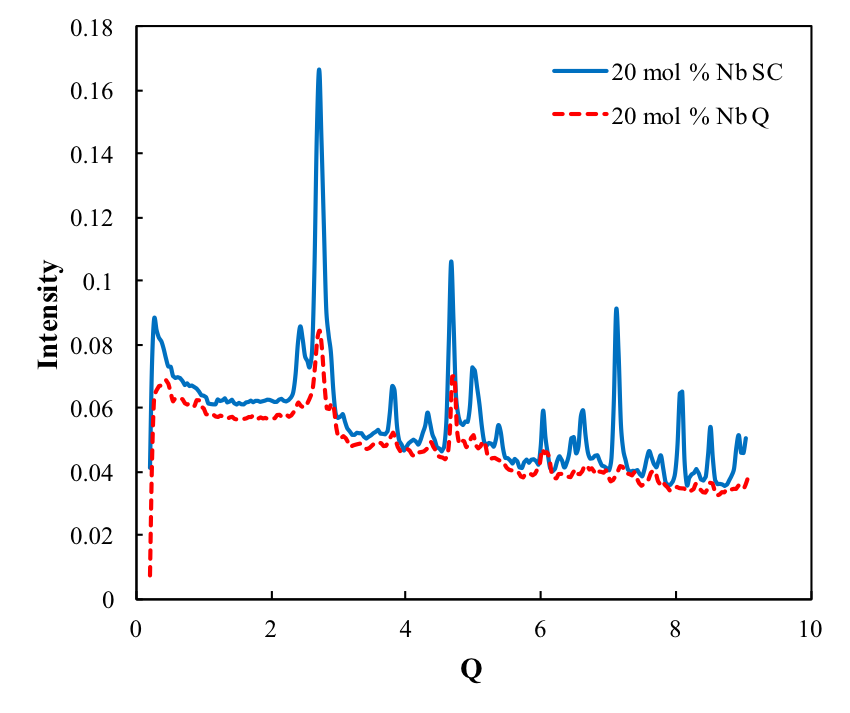
\includegraphics[width=\textwidth]{Chapter-7/Figures/50diff20.png}
	\caption{Diffraction pattern of the Ti-Nb alloy at 20 at. \% Nb. The dashed line represents the slow cooled sample while the solid line represents the quenched sample.}
	\label{Ch7-figure:50diff20}
\end{figure}

\pagebreak
\begin{figure}[H]
	\centering
	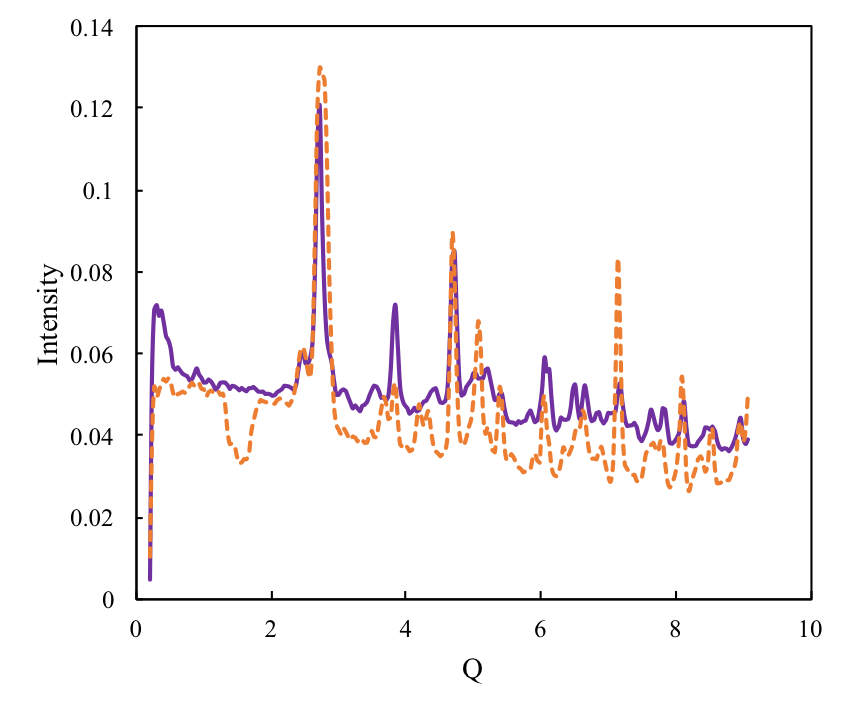
\includegraphics[width=\textwidth]{Chapter-7/Figures/50diff18.png}
	\caption{Diffraction pattern of the Ti-Nb alloy at 18 at. \% Nb. The dashed line represents the slow cooled sample while the solid line represents the quenched sample.}
	\label{Ch7-figure:50diff18}
\end{figure}

\pagebreak
\begin{figure}[H]
	\centering
	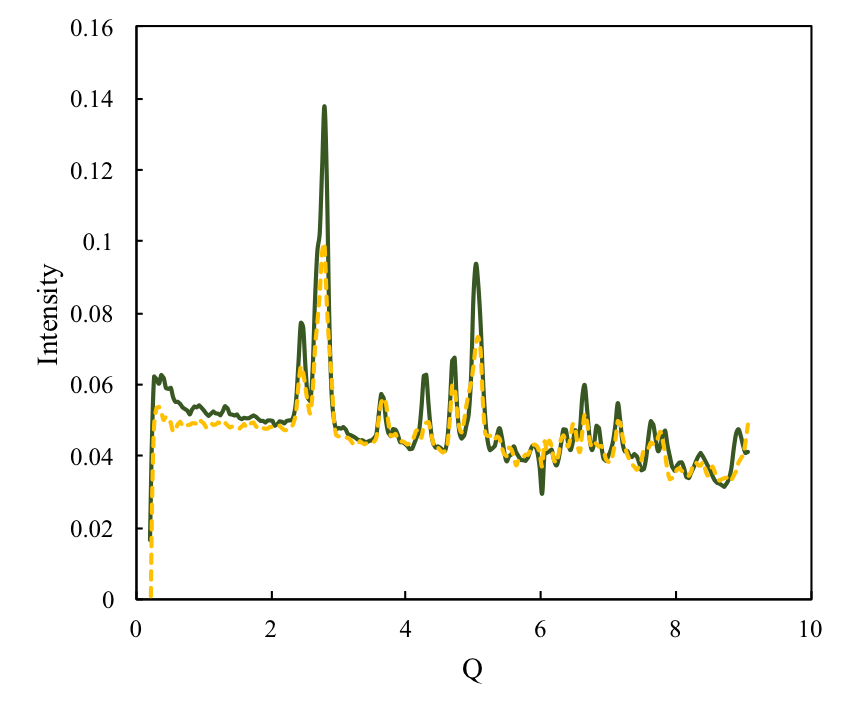
\includegraphics[width=\textwidth]{Chapter-7/Figures/50diff12.png}
	\caption{Diffraction pattern of the Ti-Nb alloy at 12 at. \% Nb. The dashed line represents the slow cooled sample while the solid line represents the quenched sample.}
	\label{Ch7-figure:50diff12}
\end{figure}

\pagebreak
\begin{figure}[H]
	\centering
	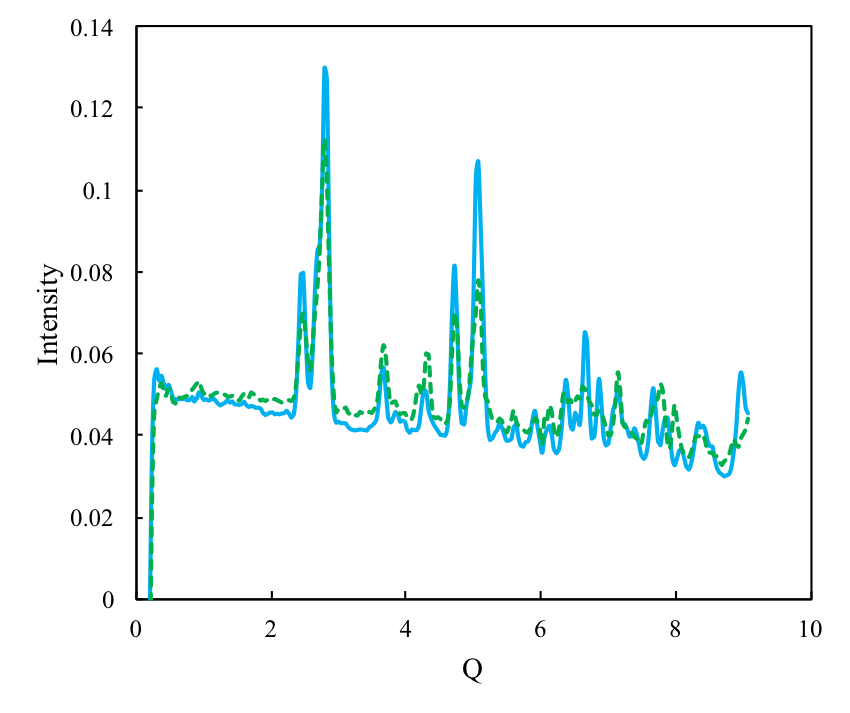
\includegraphics[width=\textwidth]{Chapter-7/Figures/50diff10.png}
	\caption{Diffraction pattern of the Ti-Nb alloy at 10 at. \% Nb. The dashed line represents the slow cooled sample while the solid line represents the quenched sample.}
	\label{Ch7-figure:50diff10}
\end{figure}